\documentclass{svproc}

\usepackage{url}
\usepackage{bm}
\usepackage{amssymb}
\usepackage{amsmath}
\usepackage{microtype}
\usepackage{hyphenat}
\usepackage{tabularx}
\usepackage{tikz}
\usetikzlibrary{arrows.meta,positioning,fit,backgrounds,calc}
\usepackage{graphicx}
\usepackage{bytefield}
\usepackage{pgfplots}
\pgfplotsset{compat=1.18}
\usepackage{algorithm}
\usepackage{algpseudocode}
\usepackage{listings}
\lstset{
  basicstyle=\ttfamily\scriptsize,
  keywordstyle=\bfseries,
  columns=fullflexible,
  showstringspaces=false,
  frame=single,
  framerule=0.4pt,
  xleftmargin=4pt,
  aboveskip=6pt, belowskip=6pt,
  numbers=none,
  breaklines=true,
}

\def\UrlFont{\rmfamily}
\makeatletter \renewcommand\@biblabel[1]{[#1]} \makeatother

\begin{document}
\mainmatter

\title{GenoID: Workload-Driven Layout Planning for Structured RFC 9562 v8 UUIDs}

\titlerunning{GenoID: Workload-Driven Layout Planning}

\author{Padala Manohar Maharshi\inst{1}$^{*}$ \and Ouku Jasmine\inst{2}}

\authorrunning{Manohar and Jasmine}

\tocauthor{Padala Manohar Maharshi and Ouku Jasmine}
\institute{Vignan's Institute Of Information Technology, Vishakhapatnam, India\\
\email{pmmaharshi@vignaniit.edu.in} \textnormal{(ORCID: 0009-0006-5807-4151)},\\
\and
Bharath Institute of Engineering and Technology, Ranga Reddy, Telangana, India \\ \email{oukujasmine@gmail.com} \textnormal{(ORCID: 0000-0002-3907-4501)}}

\maketitle              % typeset the title of the contribution

\begin{abstract}
Distributed systems need identifiers that carry application structure, a shard, a tenant, or a monotonic counter, inside a standards-compliant identifier, but RFC 9562 reserves 122 bits in version 8 without defining how to fill them, and existing generators fix field widths and positions by hand. GenoID is a declarative composition framework in which a workload-driven planner sizes fields from observed cardinality and orders them by Smith's rule, and one shared constraint-guided repair pass satisfies every declared allowed-set, range, and monotonic field. Repair runs in $O(k)$ with no redraw against the exponential expected cost of whole-identifier rejection sampling, carries a proven total-variation bound $m/2^\ell$ on allowed-set fields, and draws from pooled CSPRNG pools that are entropy-neutral by construction. Evaluation covers $10^8$-draw uniformity matching the closed form, NIST/dieharder sanity checks, cross-language byte-identity, nine-environment throughput, a $4.7\times$ workload-loop win on the hot query, and a bounded forward-secrecy analysis with by-design metadata leakage disclosed.
\keywords{distributed data systems, sharding, UUID, RFC 9562, workload-driven design, evaluation}
\end{abstract}

\section{Introduction}

RFC~9562 v8 reserves 122 bits for application structure but specifies no algorithm to fill them. GenoID fills them on the first try in $O(k)$ with no unbounded tail (one shared pass serving every layout, not a faster per-layout sampler). Version 4 carries no structure, v7 fixes one timestamp layout, and the steganographic prior art embeds one timestamp with no multi-field composition (\S\ref{sec:why-embed}--\ref{sec:composite-bench} state when embedding wins and what it costs).



\noindent\textbf{Contributions.}
\begin{itemize}
    \item Declarative RFC~9562 v8 layout abstraction for typed, constrained fields, served by one shared repair pass.
    \item Constraint-guided repair in $O(k)$ with no redraw and total-variation bound $m/2^\ell$ on allowed-set fields (exact iff $m \mid 2^\ell$); not faster than per-layout direct construction, which is equally $O(k)$ and exactly uniform.
    \item Pooled CSPRNG architecture, entropy-neutral by construction, with bounded forward-secrecy window and by-design metadata leakage disclosed.
    \item Validation at $10^8$ draws (within $0.012$ pp of the closed form), NIST/dieharder sanity checks, and nine-environment throughput, with limits disclosed.
\end{itemize}

\noindent\textbf{Organization.} Related work, layout and repair (\S\ref{sec:related-work}--\ref{sec:repair}), formal bounds and workload planning (\S\ref{sec:formal}), evaluation (\S\ref{sec:evaluation}), limits and conclusion.

\section{Related Work}
\label{sec:related-work}
\subsection{UUID standards: RFC 4122 to RFC 9562}
UUIDs originated as RFC~4122 (versions~1--5), obsoleted by RFC~9562 (2024), which adds versions~6, 7, and~8~\cite{4}. UUIDv4 carries 122 CSPRNG bits but lacks order; UUIDv7 prepends a 48-bit timestamp for index locality~\cite[\S5.7]{4}; UUIDv8 is explicitly experimental, with the RFC providing no creation algorithm for its 122 bits~\cite[\S5.8]{4}; its Appendix~B illustrates custom v8 algorithms without prescribing generation, confirming the standard leaves the design space open rather than unoccupied.
\subsection{Prior art and lineage}
RFC~9562 surveyed sixteen prior implementations~\cite{4}: ULID~\cite{5}, KSUID~\cite{6}, Snowflake~\cite{7}, TypeID~\cite{8}, COMBGUID-style sequential GUIDs, and MongoDB ObjectId, the canonical embedded-structure precedent. Time-ordered identifiers improve database behavior~\cite{9}, confirmed by academic comparisons of UUIDv4/v7/ULID~\cite{10}. All are fixed, hand-coded layouts; none offers a declarative language with per-field repair. Three systems come closest. The steganographic prior art~\cite{11}, a PostgreSQL C extension, embeds one encrypted timestamp with no multi-field abstraction. Microshard~\cite{14} is a fixed RFC~9562 version 8 with zero-lookup routing but no admissibility vocabulary, repair policy, or workload-varying random budget. Source-Known Identifiers~\cite{26} fixes three tiers with keyed origin checks where GenoID declares arbitrary fields with deterministic repair and a stated uniformity bound. GenoID concedes the fixed-layout case entirely.
Constrained-generation lineage (QuickCheck~\cite{15}, uniform constrained data~\cite{16}, generator repair~\cite{17}, synthesised generators~\cite{18}) solves arbitrary predicates; GenoID projects one fixed-width field into one admissible set with only the fibre bound. Schema languages~\cite{25} validate after the fact, while the repair pass is the generator. For locality without embedding, hash-sharded indexes~\cite{19}, randomized keys~\cite{20}, sequential GUIDs~\cite{21}, and expression indexes apply (expression index: $1.93\times$ storage at lookup parity on the same rig). Pooled draws~\cite{12} and native time-ordered functions~\cite{13} motivate the 256-entry pool.

\section{Is there a GenoID Architecture?}
\label{sec:design}
The 122 free bits are a form with labeled blanks (timestamp, shard, counter). GenoID declares the form once and fills every blank correctly on every call.

\medskip
\noindent\emph{Example:} shard~3 at time $t$: first 48 bits read as $t$, shard byte reads 3, a router extracts shard~3 directly; the rest is random.

\subsection{Declarative layout}
\label{sec:layout}
A layout declaration lists ordered fields with bit offset, length, type, and optional constraint.

Database-key declares three fields: 48-bit millisecond timestamp at offset~0, 8-bit shard at offset~52 (five admissible values), 16-bit monotonic counter at offset~66. Bits 48--51 (version) and 64--65 (variant) are reserved per RFC~9562; all other undeclared bits are random filler.

No per-layout code is written: the same pass (Algorithm~\ref{alg:repair}) serves every declaration (e.g. a 12-bit tenant plus 8-bit region enum yields the multi-tenant layout).

\begin{figure}[!ht]
\centering
\resizebox{\columnwidth}{!}{%
\begin{bytefield}[bitwidth=1.05em,boxformatting={\centering\footnotesize}]{32}
  \bitbox{32}{timestamp (bits 0--31)} \\
  \bitbox{16}{timestamp 32--47}
    \bitbox{4}{\scriptsize ver$^\dagger$}
    \bitbox{8}{shard}
    \bitbox{4}{\scriptsize rnd} \\
  \bitbox{2}{\scriptsize var$^\dagger$}
    \bitbox{16}{counter}
    \bitbox{14}{random} \\
  \bitbox{32}{random}
\end{bytefield}%
}
\caption{Database-key v8 layout as four 32-bit words. $^\dagger$RFC-fixed version/variant bits; rest: timestamp, shard, counter, random.}
\label{fig:layout}
\end{figure}

\subsection{Implementation: pooled CSPRNG generation}
\label{sec:pooled-gen}
A 256-entry pool is filled from the OS CSPRNG on first use and refilled in full when exhausted. Each call draws one 128-bit value; the shared pass (Algorithm~\ref{alg:repair}) repairs any out-of-range constrained field.

\subsection{Constraint-guided repair}
\label{sec:repair}

\begin{algorithm}[!ht]
\caption{Single-pass constraint satisfaction}
\label{alg:repair}
\begin{algorithmic}[1]
\Require Layout $L$ with fields $f_1..f_n$; candidate 128-bit value $u$
\Ensure  $u'$ satisfying every \textsc{allowed}-set and \textsc{range} constraint declared in $L$ (shipped layouts declare at most one per field; monotonic fields: Lemma~\ref{lem:counter})
\Statex
\For{each $f \in L.\textit{fields}$ with $f.\textit{constraint} \in \{\textsc{allowed},\, \textsc{range}\}$}
  \State $v \gets \textsc{ExtractBits}(u,\, f.\textit{offset},\, f.\textit{length})$
  \State $c \gets f.\textit{constraint}$
  \If{$c.\textit{kind} = \textsc{allowed}$}
    \State $v' \gets
           \begin{cases}
             v & v \in c.\textit{allowed} \\
             c.\textit{allowed}[\,v \bmod |c.\textit{allowed}|\,] & \text{otherwise}
           \end{cases}$
            \Comment{$O(1)$}
  \ElsIf{$c.\textit{kind} = \textsc{range}$}
    \State $v' \gets \max\bigl(c.\textit{min},\ \min(v,\, c.\textit{max})\bigr)$
            \Comment{$O(1)$}
  \EndIf
  \State $u \gets \textsc{WriteBits}(u,\, f.\textit{offset},\,
          f.\textit{length},\, v')$
\EndFor
\State \Return \textsc{SetVersionVariant}(u)
        \Comment{RFC~9562 \S4.2}
\end{algorithmic}
\end{algorithm}

\textbf{Lemma (tick-keyed counter).}\label{lem:counter} Monotonic fields never enter the loop: the refill path clamps time to $\max(\textit{clock}, \textit{last tick})$, increments within a tick, and stalls on exhaustion, so no emitted pair moves backwards. With $\ell_c=16$, $2^{15}$ increments/ms give $\sim10\times$ margin at 3040 UUIDs/ms; per-generator state needs no locks. Fig.~\ref{fig:pipeline}: shard 7 is repaired to 3, no redraw.

\begin{figure}[!ht]
\centering
\resizebox{0.55\columnwidth}{!}{%
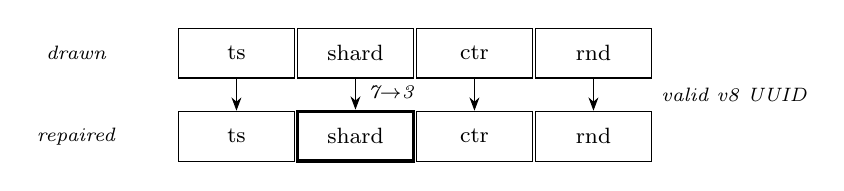
\begin{tikzpicture}[
  font=\footnotesize,
  cell/.style={draw,minimum width=42pt,minimum height=18pt,align=center},
  pick/.style={fill=black!10},
  lbl/.style={font=\scriptsize\itshape},
  >={Stealth[]}]
% Drawn candidate
\node[lbl] at (-58pt,0) {drawn};
\node[cell] (c1) at (0,0)    {ts};
\node[cell] (c2) at (43pt,0) {shard};
\node[cell] (c3) at (86pt,0) {ctr};
\node[cell] (c4) at (129pt,0){rnd};
% repair
\node[lbl] at (-58pt,-30pt) {repaired};
\node[cell] (r1) at (0,-30pt)   {ts};
\node[cell,draw=black,very thick] (r2) at (43pt,-30pt) {shard};
\node[cell] (r3) at (86pt,-30pt){ctr};
\node[cell] (r4) at (129pt,-30pt){rnd};
\draw[->] (c2) -- node[right=1pt,lbl]{\scriptsize 7$\to$3} (r2);
\draw[->] (c1) -- (r1); \draw[->] (c3) -- (r3); \draw[->] (c4) -- (r4);
\node[lbl,right] at (150pt,-15pt) {valid v8 UUID};
\end{tikzpicture}%
}
\caption{Repair: out-of-range shard 7 to admissible 3 by index-modulo. No redraw.}
\label{fig:pipeline}
\end{figure}

\section{Field and layout issues}
\label{sec:applications}
Each use below declares one layout and reads one field; no per-application generation code.

\subsection{Why embed structure in the key?}
\label{sec:why-embed}
The obvious alternative is a composite key
$(\textit{shard\_id}, \textit{uuid})$ or a separate indexed column. That
design is simpler and wins on three axes: resharding is a column update,
the identifier keeps all 122 random bits, and the shard count is unbounded
by field width. Embedding wins in one circumstance: when the identifier must
cross a boundary carrying a single value. A composite key crossing such a
boundary degrades to string concatenation: ad-hoc, unvalidated, and no longer
a UUID. A second benefit is integrity: a row whose key-embedded tenant
disagrees with its session context is impossible by construction. Never trust
the key-embedded tenant for authorization; any key holder can forge it.

Do not embed when the identifier never leaves the database, when the shard set churns, or when concealment matters: structured bits leak by design. Database-key leaves 50 random bits (50\% bound $3.95\times10^7$). Migrations version layout names with dual-generation readers; bursts above $2^{\ell_c}$/tick stall by construction.

\noindent\textbf{Deploy iff:} the key crosses a boundary alone; the shard set is stable; the residual budget fits; concealment is not required.

\subsection{Cost of embedding versus a composite key}
\label{sec:composite-bench}
Five arms run over one workload with the same timestamp-sorted 128-bit identifier, so only shard placement varies. A lookup by identifier alone cannot seek a $(\textit{shard},\textit{id})$ key (full scan); the honest comparison adds the secondary index. Embedding avoids it: $1.99\times$ less storage (28.4 vs 56.4 bytes/row), $1.88\times$ higher insert throughput, $1.29\times$ faster lookups (one index descent vs two). Inserts match the unindexed composite within 15\% ($291$K vs $250$K rows/s); point lookups match concatenated text ($11.7$ vs $12.8\,\mu$s) without leaving the UUID space. The conceded expression-index alternative costs $1.93\times$ storage for lookup parity. No claim on shard-major scans, where the composite leading column wins $3.1\times$. Native PostgreSQL/MySQL runs at $N=10^5$ show insert parity with UUIDv7; full plans are archived.

\begin{table}[t]
\caption{Schema comparison (SQLite~\cite{22}, $N=10^5$; lookup by identifier alone; means, 95\% CIs archived).}
\label{tab:composite}
\centering\scriptsize\setlength{\tabcolsep}{3pt}
\begin{tabular}{lcccc}
\hline\noalign{\smallskip}
\textbf{Schema} & \textbf{B/row} & \textbf{Ins (K/s)} & \textbf{Lookup ($\mu$s)} & \textbf{Scan (ms)} \\
\noalign{\smallskip}\hline\noalign{\smallskip}
Embedded      & \textbf{28.4} & 291 & 11.7 & \textbf{22.72} \\
PK only       & 30.2 & 250 & $\sim$6\,750 (scan) & \textbf{7.38} \\
PK $+$ index  & 56.4 & 155 & 15.1 & 5.73 \\
Text key      & 52.4 & 234 & 12.8 & 21.24 \\
PK $+$ expr idx & 54.9 & 141 & 12.2 & 30.62 \\
\noalign{\smallskip}\hline
\end{tabular}
\end{table}

\subsection{Sharded databases}
The database-key embeds the shard; a router extracts bits 52--59 with a bit-mask, replacing hash plus ring lookup. \label{sec:cluster} On one host (4 cores, SQLite shard files, 100K identifiers over shards 1--5) the full five-shard sweep is $11.89$\,ms vs $22.72$\,ms for the single-index scan ($1.91\times$); a versioned reshard (shards 6--8) migrates at 51{,}939 rows/s with $1.52\times$ dual-read overhead. One-host only: no network, replication, or skew; cross-node behaviour is future work.

\subsection{More layouts}
The same pattern covers multi-tenancy (12-bit tenant, 8-bit region; residency without a secondary index) and event sourcing (16-bit node plus 24-bit counter; ordered logs without a sequence server).

\section{Formal Analysis}
\label{sec:formal}
Rejection gambles on a lucky whole-UUID draw; repair fixes only the fields that need it, at no entropy cost.

\subsection{Repair complexity: $O(k)$ versus an expected $64^k$ draws}
\label{sec:repair-complexity}

\textbf{Setup.} For $k$ fields with $a_i$ values in $\ell_i$ bits, rejection needs $\prod_i 2^{\ell_i}/a_i$ draws expected. At $a_i=4$, $\ell_i=8$ (density $2^{-6}$, near the $5/256$ shard field) this is $64^k$ ($6.9\times10^{10}$ at $k=6$) with no upper bound on any run. Repair (Algorithm~\ref{alg:repair}) iterates once with $O(1)$ branches, so worst-case $O(k)$ with no redraws. Per-layout direct construction is equally $O(k)$ and exactly uniform; repair wins by serving every layout with one shared pass, not by beating it. The $64^k$ figure is one representative cell.

\subsection{Entropy preservation}
\label{sec:entropy}

A pooled draw is distributionally identical to a direct CSPRNG call, so pooling is measure-preserving. Repair is deterministic, so $H(g(X)) \leq H(X)$: it never adds entropy. Pooled and unpooled variants pass NIST identically (\S\ref{sec:nist}).

\subsection{Uniformity of constraint repair}
\label{sec:uniformity}

Let $A = (a_0, a_1, \dots, a_{m-1})$ be the admissible set in declaration order, $m = |A|$, and let $C_i = \left\lfloor (2^\ell - 1 - i)/m \right\rfloor + 1$ be the number of $\ell$-bit values congruent to $i$ modulo $m$. Index-modulo repair sends a raw value $v$ to $a_{v \bmod m}$, so the fibre of $a_i$ is exactly $C_i$. The load-bearing claim is exact uniformity iff $m \mid 2^\ell$ (Theorem below); the envelope is bounded by
\[
  \|p - u\|_{\mathrm{TV}} \;\le\; \frac{m}{2^\ell}, \qquad
  \max_i |p(a_i) - 1/m| \;\le\; \frac{\lceil 2^\ell/m \rceil}{2^\ell},
\]
where $u$ is uniform on $A$.

\textbf{Theorem (fibre sizes).} On the compiled path, which applies $A[v \bmod m]$ unconditionally, the probability of drawing $a_i$ is $C_i / 2^\ell$, and the repaired distribution is exactly uniform \emph{iff} $m \mid 2^\ell$.

The pooled path keeps an already-admissible value as itself before falling back to $A[v \bmod m]$, so it partitions the raw values differently. Writing $G_i = |\{a \in A : a \equiv i \pmod m\}|$, the fibre of $a_i$ on that path is $1 + C_i - G_i$. The two agree on every contiguous admissible set, and differ as soon as the set skips a residue class.

\textbf{Corollary (pooled-path uniformity).} On the pooled path the repaired distribution is exactly uniform \emph{iff} $m \mid 2^\ell$ and $G_i = 1$ for every $i$, i.e.\ the admissible set occupies every residue class exactly once.

Both conditions hold for every evaluated layout. Database-key ($m=5$, $\ell=8$) holds $(52,51,51,51,51)$ values (max deviation $0.31\%$); multi-tenant fields satisfy $m \mid 2^\ell$, $G_i=1$ and are exactly uniform. The \textsc{range} branch clamps and is not uniformity-preserving; neither evaluated layout declares one. Endpoint masses match within $0.06$ pp ($4/4$ cells), fibres within $0.3$ pp ($24/24$ cells; archived grid).

\subsection{Bit allocation}
\label{sec:bit-allocation}

Width is an entropy question, position a locality one. A field with $c$ values needs $\lceil \log_2 c \rceil$ bits; $n$ identifiers need residual $r=\lceil \log_2\, n(n-1)\,/\,4\ln\frac{1}{1-\tau} \rceil$ (47 bits for $2$M at $\tau=10^{-2}$). Over-budget declarations are refused. Weighted depth $D=\sum_i w_i(o_i+\ell_i)$ is the single-machine weighted-completion-time objective, so Smith order ($w_i/\ell_i$ descending~\cite{24}) is exact on one segment and near-optimal across reserved bits. \begin{table}[t]
\caption{Bit allocation vs exhaustive optimum and role-rank order.}
\label{tab:bit-allocation}
\centering\scriptsize\setlength{\tabcolsep}{3pt}
\begin{tabular}{lcc}
\hline\noalign{\smallskip}
\textbf{Quantity} & \textbf{Value} & \textbf{Basis} \\
\noalign{\smallskip}\hline\noalign{\smallskip}
Exhaustive optimum hit & 495/500 & 99.0\% \\
Suboptimal (cross bit~48) & 5/500 & 0.39--2.40\% \\
Role-rank worse & 418/500 & gap 23.26\% \\
Cost per bit & $\approx 95$ in $D$; $\times 2$ coll. \\
Dbkey struct / residual & 67 / 55 bits & needs 47 \\
\noalign{\smallskip}\hline
\end{tabular}
\end{table}

The allocator is optimal on one free segment and within a few percent across reserved bits. The shipped declaration is already optimal (the 8-bit shard wastes five residual bits). Smith's rule is from 1956; the contribution is the reduction plus the collision-safety constraint.

\subsection{Closing the loop: workload-driven weights}
\label{sec:workload-planning}

Workload inference recovers weights (access counts), roles (range-filtered to partition, point-filtered to lookup), and cardinality from a seeded 10K-query trace; Smith order places the hot field first. On 200K-row SQLite tables the tenant-heavy mix infers weights 7987/1530, puts tenant first, and wins $3099$ vs $14694\,\mu$s per lookup ($4.7\times$, 5 reps of 500, non-overlapping CIs) at insert parity; the inverted mix converges to the hand layout at parity. The trace is synthetic but seeded and archived; a skewed trace is favourable by construction, \S\ref{sec:composite-bench} stands for the neutral case.

\subsection{Microshard head-to-head}
\label{sec:microshard}

Closest overlap Microshard (fixed v8: 54-bit time, 32-bit shard, 36 random bits; bit-exact mirror cross-checked) wins modestly for the prunable layout on the same 200K-row setup with parity elsewhere (numbers archived). 

\section{Confidentiality and Authentication}
\label{sec:security}

The OS CSPRNG is assumed reliable, matching RFC~9562 \S8. Every GenoID pool refill is seeded from it. The analysis considers passive observers, state compromise, structure inference, and collision attacks.

\subsection{Entropy accounting}
\label{sec:entropy-accounting}

\begin{table}[t]
\caption{Structural entropy budget.}
\label{tab:min-entropy}
\centering\scriptsize\setlength{\tabcolsep}{3pt}
\begin{tabular}{lccc}
\hline\noalign{\smallskip}
\textbf{Generator} & \textbf{Bits} & \textbf{Secret} & \textbf{Entropy} \\
\noalign{\smallskip}\hline\noalign{\smallskip}
UUIDv4 & 128 & 122 random & 122 \\
UUIDv7 & 128 & 74 random & 74 \\
GenoID v8 & 128 & 122 CSPRNG & 122 \\
GenoID dbkey & 128 & 50 random & 50 \\
Others$^\dagger$ & 128 & 0--122 & 0--122 \\
\noalign{\smallskip}\hline
\end{tabular}
\smallskip
\scriptsize $^\dagger$ULID-v8, pg\_uuid\_v8, non-crypto (runtime PRNG, not a CSPRNG).
\end{table}

Database-key keeps $128-48-8-16-6=50$ random bits; residual security is that of the 50-bit payload. Structured layouts leak metadata by design (the steganographic prior art masks timestamps). The counter is predictable within a tick by design (RFC~9562 \S6.2). Pools hold 256 (base) to 1024 (structured) entries; a state compromise predicts at most 1024 future UUIDs per generator (bounded forward secrecy); past buffers are overwritten. 


\section{Evaluation}
\label{sec:evaluation}
Throughput is stated as same-rig relative ratios over nine environments (three OS by three runtimes), not cross-host absolutes; every result maps to its harness in Table~\ref{tab:artifact-map}. RQ1 composition (\S\ref{sec:composition-correctness}), RQ2 repair cost (\S\ref{sec:repair-vs-rejection}), RQ3 uniformity/collisions/batteries, RQ4 throughput and database behaviour.

\subsection{Composition correctness}
\label{sec:composition-correctness}
Over 1.5M structured-field checks on the shipped production path: 0 mismatches, 0 constraint violations, 0 monotonicity violations.

\subsection{Repair versus rejection cost}
\label{sec:repair-vs-rejection}

Over 40 $(d,k)$ cells, repairs per identifier follow $k(1-d)$ (exactly $k$ as $d \to 0$); rejection follows $d^{-k}$ ($64^k$ reproduced at $d=1/64$ for $k=3,4,6$). Rejection wins for one loosely constrained field; GenoID wins when constraints are tight, many, or tail latency must be bounded (absolute timings archived; warm-up noted in \S\ref{sec:validity}).

\subsection{Collision and uniformity}
Over $10^8$ database-key draws, shard frequencies match the closed form ($52/256$ once, $51/256$ four times) within $0.012$ pp ($2.9$ binomial SD at $0.004$ pp); multi-tenant fields within $0.008$ pp. No value ever leaves its declared set in $2\times10^8$ draws. Database-key collisions use 50 payload bits (50\% bound $3.95\times10^7$). A non-crypto generator passes the same 1M-draw gate in all nine environments, confirming the gate has no discriminating power.

\subsection{NIST SP 800-22 and dieharder}
\label{sec:nist}
Structural sanity check only, not certification: SP~800-22 is withdrawn, five streams per layout (NIST prefers $\geq 100$). Full battery ran on all three layouts ($10^7$-bit exports); curated dieharder subset reports modal PASS on all 152 rows (unstructured and database-key payloads; full tables archived).

\subsection{Throughput and baseline comparison}
\label{sec:throughput}

The loop consumes every identifier (unconsumed loops overstated pure-JS rates by $\sim2\times$). Only same-rig ratios are claimed.

\begin{table}[t]
\caption{Throughput over nine environments (M UUIDs/s; means, 95\% CIs archived; same-rig ratios claimed).}
\label{tab:throughput}
\centering\scriptsize\setlength{\tabcolsep}{3pt}
\begin{tabular}{lcc}
\hline\noalign{\smallskip}
\textbf{Generator} & \textbf{Rep env} & \textbf{Range, 9 envs} \\
\noalign{\smallskip}\hline\noalign{\smallskip}
Platform random   & 16.48 & 3.15--31.34 \\
Snowflake$^\dagger$ & 3.63 & 3.10--8.55 \\
Pooled            & 3.15 & 2.73--5.84 \\
Compiled struct   & 0.95 & 0.19--1.18 \\
Interpreted struct & 0.91 & 0.31--1.16 \\
Hand-coded        & 2.60 & 0.38--3.95 \\
Baseline B        & 1.04 & 0.23--1.39 \\
Stego prior art   & 0.47 & 0.19--0.58 \\
Other baselines   & 0.34--0.50 & 0.08--0.86 \\
\noalign{\smallskip}\hline
\end{tabular}
\smallskip
\scriptsize $^\dagger$64-bit time+sequence, excluded from the collision gate (sequence wraps under tight loops).
\end{table}

\begin{table}[t]
\caption{Same-rig ratios vs the two structured baselines (n.s.: $p>0.05$; all 18 clear $p<0.05$, detail archived).}
\label{tab:paired}
\centering\scriptsize\setlength{\tabcolsep}{3pt}
\begin{tabular}{lccc}
\hline\noalign{\smallskip}
\textbf{Env} & \textbf{vs prior art} & \textbf{vs baseline B} & \textbf{comp/interp} \\
\noalign{\smallskip}\hline\noalign{\smallskip}
A & 1.92$\times$ & 0.87$\times$ & 1.05 \\
B & 2.67$\times$ & 0.76$\times$ & 0.97 (n.s.) \\
C & 2.48$\times$ & 1.17$\times$ & 1.02 (n.s.) \\
D & 1.52$\times$ & 1.37$\times$ & 0.67 \\
E & 0.76$\times$ & 0.79$\times$ & 0.76 \\
F & 1.62$\times$ & 1.36$\times$ & 0.63 \\
G & 1.93$\times$ & 1.53$\times$ & 0.93 \\
H & 1.50$\times$ & 1.08$\times$ & 1.07 (n.s.) \\
I & 1.74$\times$ & 1.33$\times$ & 0.94 \\
\noalign{\smallskip}\hline
\end{tabular}
\end{table}

Structured leads the steganographic prior art in eight of nine environments and the second baseline in seven ($1.1$--$2.7\times$ where ahead; Table~\ref{tab:paired}, all $p<0.05$). A hand-coded time-ordered variant is faster everywhere ($0.27$--$0.82\times$ for structured) but expresses no declared constraints. Snowflake is faster ($3.0$--$21.6\times$) as a 64-bit integer across guarantee classes. The compiled path regresses on one runtime ($0.63$--$0.76\times$); interpreted structured runs at $0.06$--$0.37\times$ of pooled base.

\subsection{Ablation}
\label{sec:ablation}
The inlined-code compiler is not shipped: parity on two runtimes, $0.63$--$0.76\times$ regression on the third, so the interpreted pass is the portable default. The two-parent design is load-bearing ($6.3\times$ throughput vs single-parent at identical quality; archived E7).

\subsection{Additional deployability checks}
\label{sec:deployability}
Concurrent generation: 0 cross-worker collisions. SQLite B-tree (500K rows): structured inserts at $90.3$K rows/s vs $61.5$K (v7) vs $7.0$K (v4) at equal density. Cross-browser (three engines): 0 errors, 0 collisions.

\subsection{Cross-language reproducibility}
\label{sec:cross-lang}

The composition core was reimplemented in a second language: 1000 fixed-seed UUIDs per layout across three layouts match golden files byte-for-byte (3000/3000). Mutants (shifted repair, frozen counter) fail exactly the layouts declaring those constraints. Production ports use their own OS CSPRNG; fixed seeds exist only for verification.

\subsection*{Availability}
Code, harnesses, artifacts, golden vectors, and cross-language check: \url{https://github.com/mmmmaharshi/geno-id} (MIT). Table~\ref{tab:artifact-map} maps results to harnesses. This manuscript adds workload planning, the composite-key experiment, native-engine validation, and the Microshard comparison. Earlier release DOIs are deliberately uncited (they predate the monotonicity fix, E1 rewrite, and $10^8$ histogram).

\begin{table}[t]
\caption{Artifact map: result $\to$ harness and archive.}
\label{tab:artifact-map}
\centering\scriptsize\setlength{\tabcolsep}{3pt}
\begin{tabular}{lll}
\hline\noalign{\smallskip}
\textbf{Result} & \textbf{Harness} & \textbf{Archive} \\
\noalign{\smallskip}\hline\noalign{\smallskip}
E1 composition & production check & production rec \\
Repair, grids, histogram & sweep/grid/hist & sweep, grid, counts \\
Alloc, workload, microshard & alloc/workload/h2h & alloc, workload, h2h \\
NIST, dieharder & export+battery & battery, draws, dieharder \\
Throughput and DB & matrix+harnesses & consolidated, per-arm \\
Cross-language & golden export & golden files \\
\noalign{\smallskip}\hline
\end{tabular}
\end{table}

\section{Threats to Validity}
\label{sec:validity}
Deploy rule: embed when the key must cross a boundary alone, else keep the composite key. Reusable unit is the layout declaration; the fibre bound prices each declaration in advance.

\textbf{External validity.} Byte-identical reimplementation (3000 UUIDs, three layouts). Shared runners, so relative comparisons only. One-host cluster only; no cross-node dispatch, replication, or skew.

\textbf{Validity.} NIST PASS is necessary, not sufficient, for security. Numbers post-date the dead-code fix. Interpreted path runs at $0.06$--$0.37\times$ of base; deploy it on the regressed runtime. Welch $t$-tests throughout.

\section{Conclusion and Future Work}
\label{sec:conclusion}
RFC~9562 leaves v8's 122 bits undefined; GenoID fills them declaratively and portably. One shared repair pass gives $O(k)$ repair with bound $m/2^\ell$, validated at $10^8$ scale with security analysis and cross-language check. Throughput leads the steganographic prior art in eight of nine environments ($1.1$--$2.7\times$ where ahead); the primary result is making shard, tenant, and sequence identity a property of the key.

\section*{Appendix: archived supplement}
NIST per-draw tables, dieharder fractions, repair grids, worked uniformity example ($m=2$, $\ell=2$), rejection crossovers, Smith proof, Microshard detail, and family-wise assessment are archived with the battery, grid, sweep, and head-to-head records. Head-draw summary: all 123 p-values satisfy $p \geq 0.01$ ($1.1\%$ failure over five draws, Type-I noise); Spectral repeat (2/5 on multitenant) follows up 1/30, 0/30, 1/30 at $10^6$ bits.

\noindent\textbf{Supplement detail (one paragraph).}
The bound is measured directly: over four $(\ell,\textit{min},\textit{max})$ cells including the shipped conformance window ($2\times10^5$ seeded draws per cell), every measured endpoint mass matches its closed form to within $0.06$ percentage points ($4/4$ cells; the archived grid). The fibre prediction is also checked directly over a grid of $(m,\ell)$ pairs ($m \in \{2,3,4,5,8\}$, $\ell \in \{3,4,8,12,16\}$, $2\times10^5$ seeded draws per cell): every measured frequency matches its closed-form fibre to within $0.3$ percentage points ($24/24$ cells; the archived grid).

Tight example $m=2$, $\ell=2$, $A=\{0,2\}$: compiled stays $(50\%,50\%)$, pooled folds to $(25\%,75\%)$.

Database-key is $(52,51,51,51,51)$ ($0.31\%$ max deviation); multi-tenant fields are exactly uniform.

\noindent\textbf{Crossovers.} Rejection wins only for loose low-$k$ fields; boundary moves toward higher $d$ with $k$ (archived sweep).

\noindent\textbf{Smith optimality proof.}
Smith: $D$ is minimised by ordering fields in non-increasing $w_i/\ell_i$: swapping an adjacent inverted pair changes $D$ by $\ell_a \ell_b (w_a/\ell_a - w_b/\ell_b) \le 0$.

\noindent\textbf{Microshard measurement detail.}
On the same
200{,}000-row SQLite setup, a tenant prune is one PK range seek for the
tenant-first GenoID layout against a full scan with in-app shard filtering
for microshard:
$3446\,\mu$s versus $4383\,\mu$s (means over 5 reps of 500 lookups; CIs
nearly touch), with full-ID
point lookups and inserts at parity.

\noindent\textbf{Family-wise uniformity assessment.}
Across all 17 tested cells the family-wise assessment gives max-$|z|=2.90$ against a Bonferroni critical value of $2.97$ at family-wise $\alpha=0.05$ (\v{S}id\'ak $2.97$, Bonferroni $p=0.064$), i.e.\ consistent with sampling noise once the 17-fold multiple comparison is accounted for. The archived max-z analysis supports that reading, computed from the archived per-cell counts with no new draws.

\begin{thebibliography}{00}

\bibitem{1}
L. E. Bassham, A. L. Rukhin, J. Soto, J. R. Nechvatal, et al., ``A Statistical Test Suite for Random and Pseudorandom Number Generators for Cryptographic Applications,'' NIST SP~800-22 Rev.~1a, Apr.~2010 (withdrawn).

\bibitem{2}
NIST Crypto Publication Review Board, ``Decision to Revise NIST SP~800-22
Rev.~1a,'' Apr.~2022.
\url{https://www.nist.gov/news-events/news/2022/04/decision-revise-nist-sp-800-22-rev-1a}

\bibitem{3}
R. G. Brown, ``Dieharder: A Random Number Test Suite,'' Duke University, 2007. \url{https://webhome.phy.duke.edu/~rgb/General/dieharder.php}

\bibitem{4}
K. Davis, B. Peabody, and P. Leach, ``Universally Unique IDentifiers (UUIDs),'' RFC 9562, Internet Engineering Task Force (IETF), May 2024.

\bibitem{5}
A. B. Peabody, ``ULID Specification.'' \url{https://github.com/ulid/spec}

\bibitem{6}
Segment, ``KSUID.'' \url{https://github.com/segmentio/ksuid}

\bibitem{7}
Twitter, ``Snowflake.'' \url{https://github.com/twitter-archive/snowflake}

\bibitem{8}
Jetify, ``TypeID.'' \url{https://github.com/jetify-com/typeid}

\bibitem{9}
J. Nilsson, ``The cost of GUIDs as primary keys,'' InformIT, 2002.

\bibitem{10}
N. Karimian Kakolaki, ``A comparative analysis of identifier schemes: UUIDv4, UUIDv7, and ULID for distributed systems,'' arXiv:2509.08969, Sep.~2025.

\bibitem{11}
ineron, ``pg\_uuid\_v8: PostgreSQL extension for steganographic UUIDs,'' May 2026. \url{https://github.com/ineron/pg_uuid_v8}

\bibitem{12}
pscheid92, ``uuid: Go implementation of RFC 9562 with V8 and pooled/batch APIs.'' \url{https://pkg.go.dev/github.com/pscheid92/uuid}

\bibitem{13}
PostgreSQL Global Development Group, ``UUID functions,'' PostgreSQL~18 Documentation. \url{https://www.postgresql.org/docs/current/functions-uuid.html}

\bibitem{14}
dilipvamsi, ``microshard-uuid: RFC 9562 v8 with zero-lookup routing.'' \url{https://github.com/dilipvamsi/microshard-uuid}

\bibitem{15}
K. Claessen and J. Hughes, ``QuickCheck: a lightweight tool for random testing of Haskell programs,'' Proc.\ ICFP, 2000. \url{https://doi.org/10.1145/1988042.1988046}

\bibitem{16}
K. Claessen, J. Dureg{\aa}rd, and M. H. Pa{\l}ka, ``Generating constrained random data with uniform distribution,'' J.\ Functional Programming, vol.\ 25, e15, 2015. \url{https://doi.org/10.1017/S0956796815000098}

\bibitem{17}
P. LaFontaine, Z. Cao, A. Head, and J. C. Foster, ``We've Got You Covered: type-guided repair of incomplete input generators,'' Proc.\ OOPSLA, 2025. \url{https://doi.org/10.1145/3763158}

\bibitem{18}
H. Goldstein, B. C. Pierce, et al., ``The search for constrained random generators,'' Proc.\ PLDI, 2026. \url{https://doi.org/10.1145/3808329}

\bibitem{19}
Cockroach Labs, ``Hash-sharded indexes.'' \url{https://www.cockroachlabs.com/docs/stable/hash-sharded-indexes}

\bibitem{20}
PingCAP, ``AUTO\_RANDOM.'' \url{https://docs.pingcap.com/tidb/stable/auto-random/}

\bibitem{21}
Microsoft, ``NEWSEQUENTIALID.'' \url{https://learn.microsoft.com/en-us/sql-server/t-sql/functions/newsequentialid-transact-sql}

\bibitem{22}
SQLite Consortium, ``SQLite.'' \url{https://sqlite.org/}

% 23 merged into native-results note
\bibitem{24}
W. E. Smith, ``Various optimizers for single-stage production,'' Naval Research Logistics Quarterly, vol.\ 3, nos.\ 1--2, pp.\ 59--66, 1956.

\bibitem{25}
Google, ``Protocol Buffers documentation: overview.'' \url{https://protobuf.dev/overview/}

\bibitem{26}
D. S. K{\i}l{\i}c{c}, ``Source-Known Identifiers: a three-tier identity system for distributed applications,'' arXiv:2604.00151 [cs.DC], v3, Sep.~2026. \url{https://arxiv.org/abs/2604.00151}

% 27 dropped (uncited background)
\end{thebibliography}


\end{document}
